\section{Host Recovery: Descubrimiento de dispositivos}
Con ayuda de Nessus, se realizó un escaneo rápido de puertos (\textit{Host Recovery}), con la siguiente configuración:
\begin{figure}[H]
	\centering
	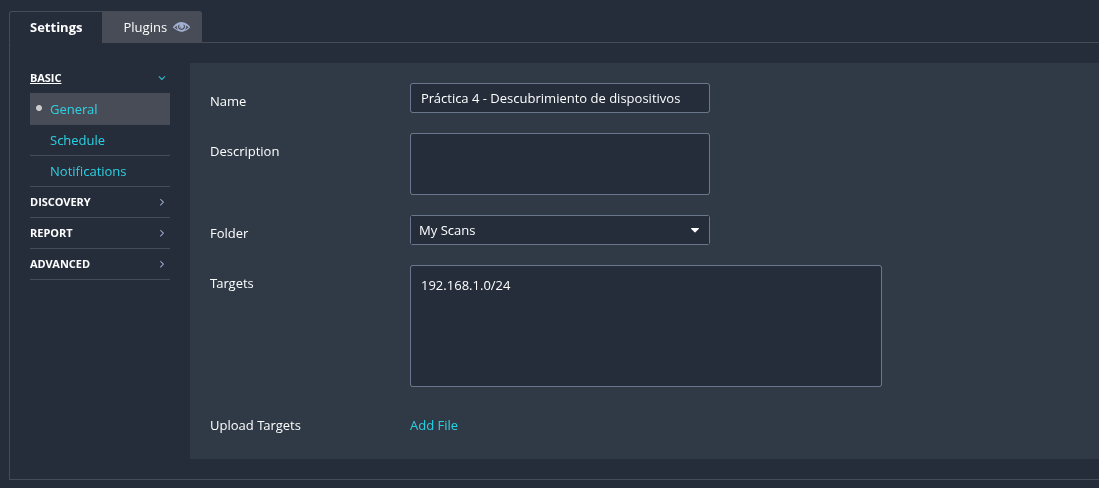
\includegraphics[scale=0.4]{imagenes/Capturas/1.png}
	\label{fig:ipCentralOps}
\end{figure}
\begin{figure}[H]
	\centering
	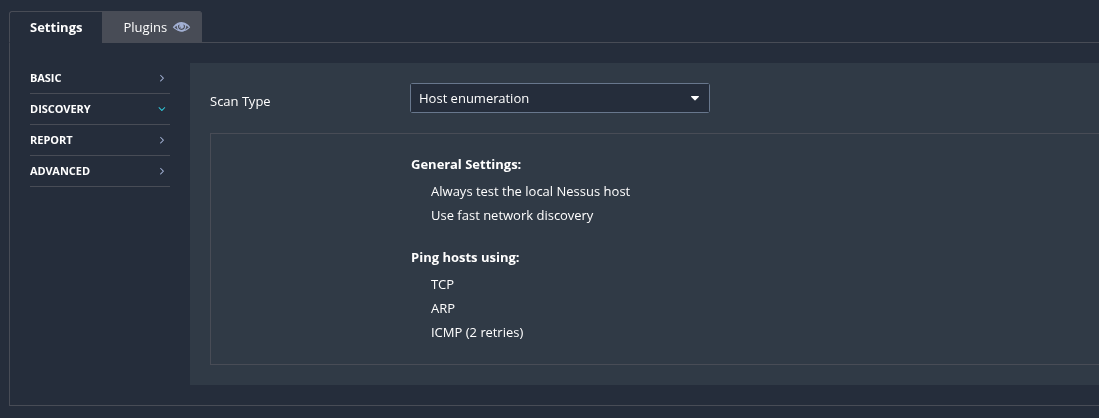
\includegraphics[scale=0.4]{imagenes/Capturas/2.png}
	\label{fig:ipCentralOps}
\end{figure}
\begin{figure}[H]
	\centering
	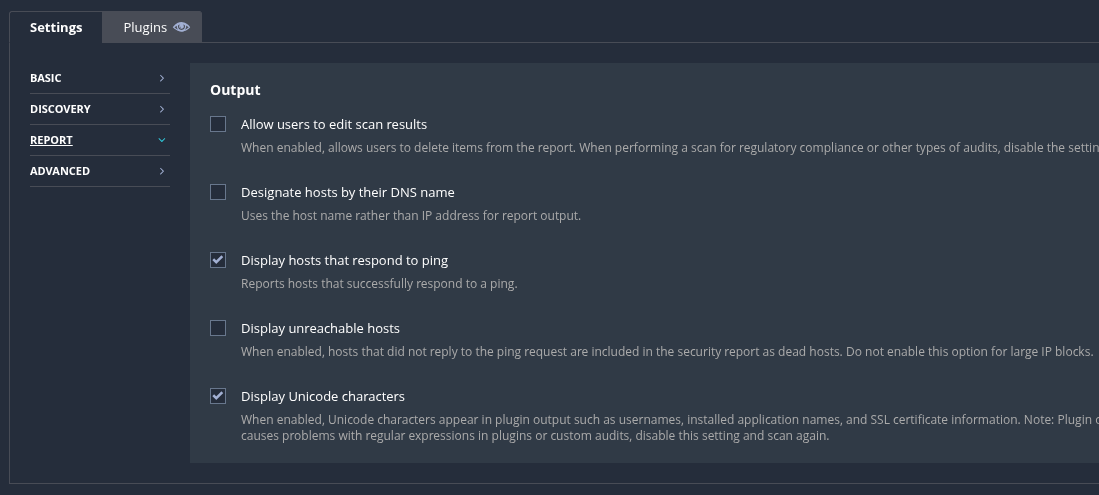
\includegraphics[scale=0.45]{imagenes/Capturas/3.png}
	\label{fig:ipCentralOps}
\end{figure}

El reporte nos muestra los siguientes puertos:
\begin{itemize}
	\item 192.168.1.65
	\item 192.168.1.67
	\item 192.168.1.68
	\item 192.168.1.113
	\item 192.168.1.160 (mi dispositivo)
	\item 192.168.1.254
\end{itemize}

Los resultados detallados de este escaneo se encuentran en el archivo \texttt{\textbf{Descubrimiento de Dispositivos.pdf}}

\newpage
\section{Basic Network Scan: Descubrimiento de vulnerabilidades}
\subsection{Primer escaneo}
Con la opción \textit{Basic Network Scan}, realizaremos un escaneo a mi equipo personal (192.168.1.160). Los parámetros del escaneo son los siguientes:
\begin{figure}[H]
	\centering
	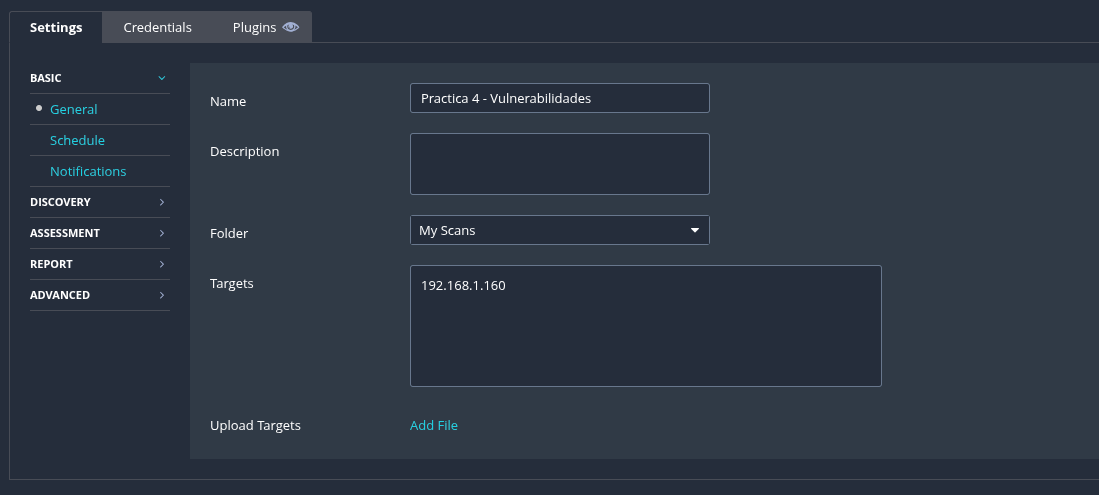
\includegraphics[scale=0.45]{imagenes/Capturas/4.png}
\end{figure}
\begin{figure}[H]
	\centering
	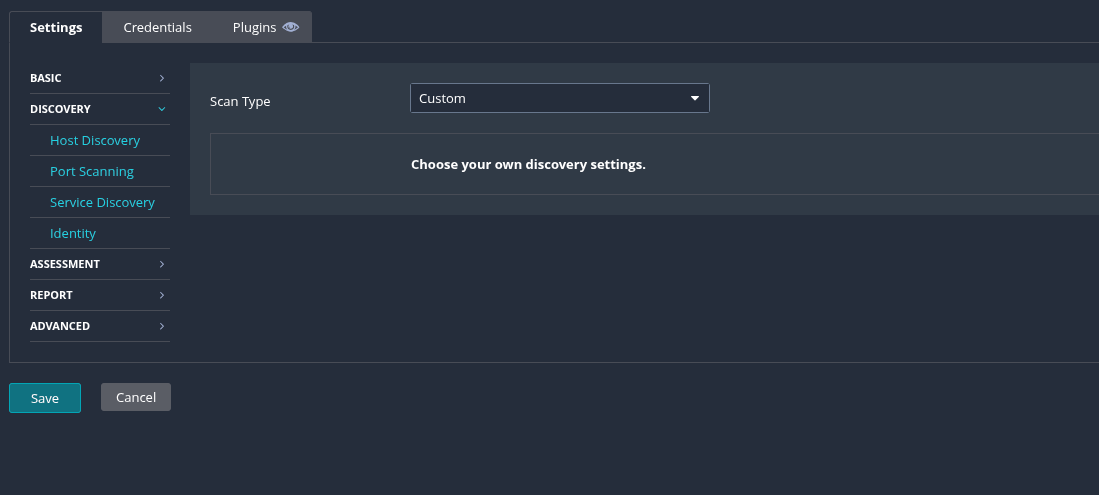
\includegraphics[scale=0.45]{imagenes/Capturas/5.png}
\end{figure}
\begin{figure}[H]
	\centering
	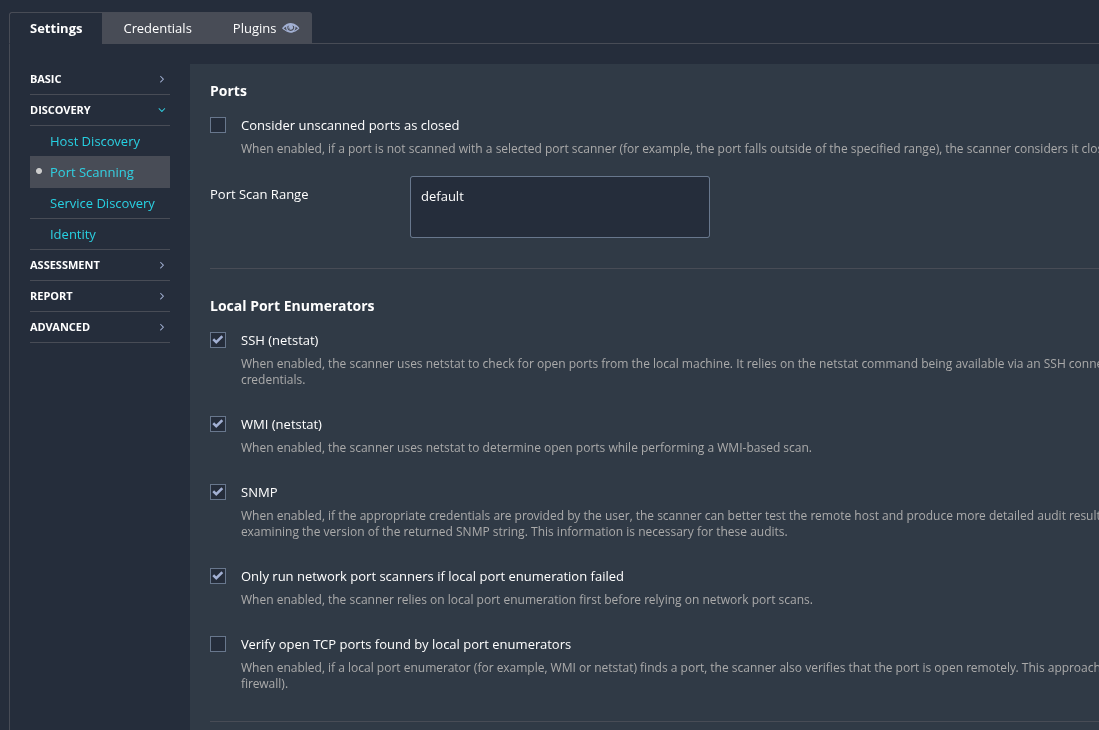
\includegraphics[scale=0.45]{imagenes/Capturas/6.png}
\end{figure}
\begin{figure}[H]
	\centering
	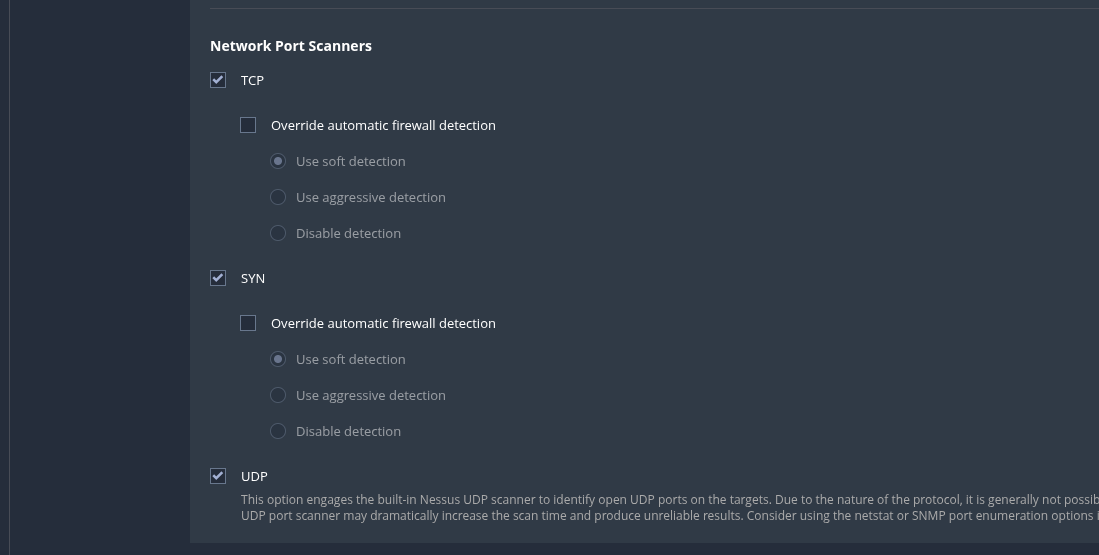
\includegraphics[scale=0.45]{imagenes/Capturas/7.png}
\end{figure}
\begin{figure}[H]
	\centering
	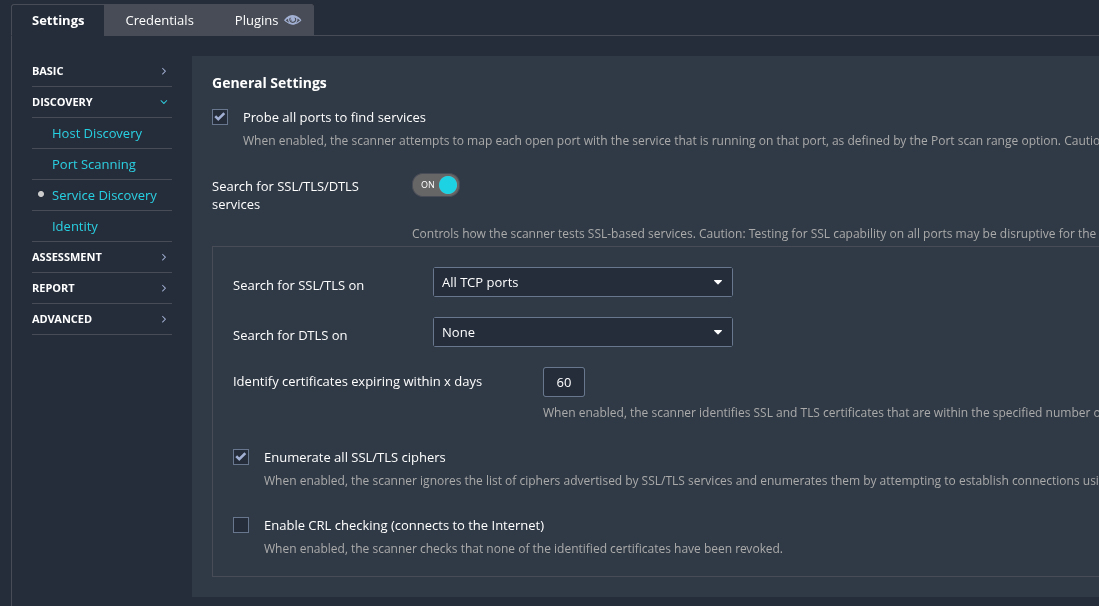
\includegraphics[scale=0.45]{imagenes/Capturas/8.png}
\end{figure}
\begin{figure}[H]
	\centering
	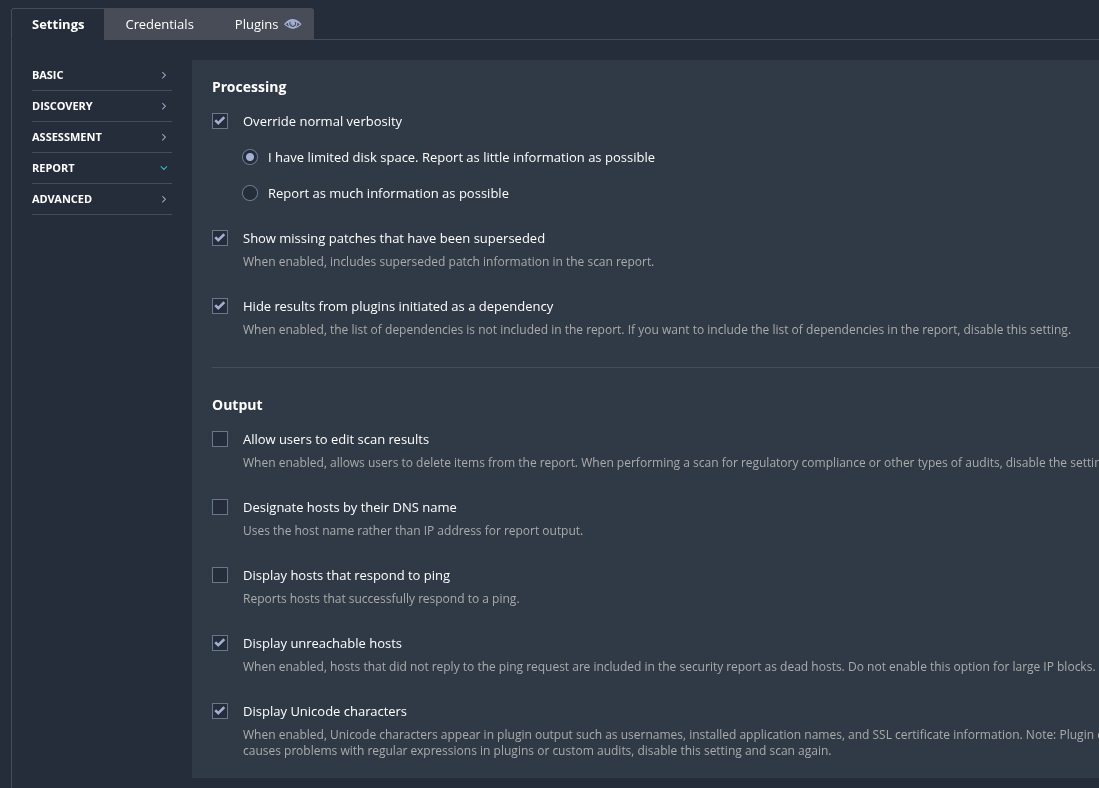
\includegraphics[scale=0.45]{imagenes/Capturas/9.png}
\end{figure}
\begin{figure}[H]
	\centering
	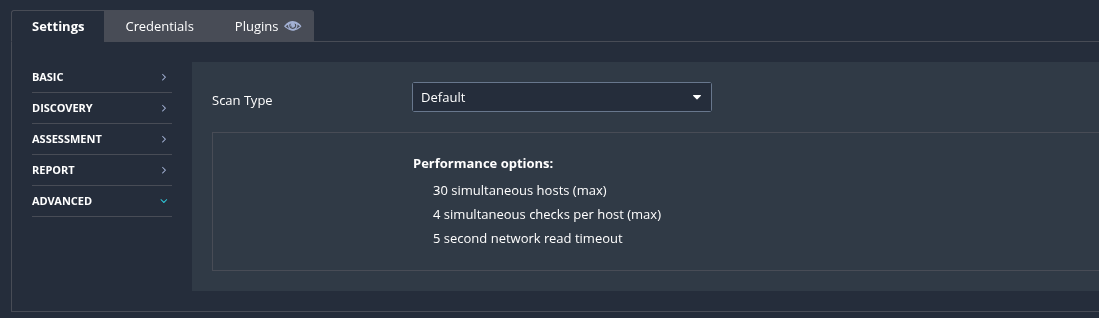
\includegraphics[scale=0.45]{imagenes/Capturas/10.png}
\end{figure}

Lo más destacado de este escaneo, es que se tiene un total de 8 vulnerabilidades Altas, 10 Medias y 3 Bajas. Estas vulnerabilidades se pueden agrupar de la siguiente forma:
\begin{itemize}
	\item \textbf{Sistema Operativo}: El sistema Fedora 38 ha llegado a su fin de vida útil. Esta es la vulnerabilidad más importante, ya que significa que los repositorios oficiales ya no reciben parches de seguridad, lo que provocando lo mismo en el resto de tus paquetes.
	\item \textbf{Res y Bases de Datos}: OpenSSH (m)últiples vulnerabilidades incluyendo RCE y ataques MitM), PostgreSQL (Heap Buffer Overflow).
	\item \textbf{Entornos de desarollo y análisis de datos}: Python (bibliotecas desactualizadas), R (vulnerabilidad de deserialización), Apache e Intel Media SDK.
	\item \textbf{Certificado SSL}: Esto se detectó en el puerto 8834. Ese es el puerto del propio Nessus. Omitiremos está vulnerabilidad.
\end{itemize}

\begin{figure}[H]
	\centering
	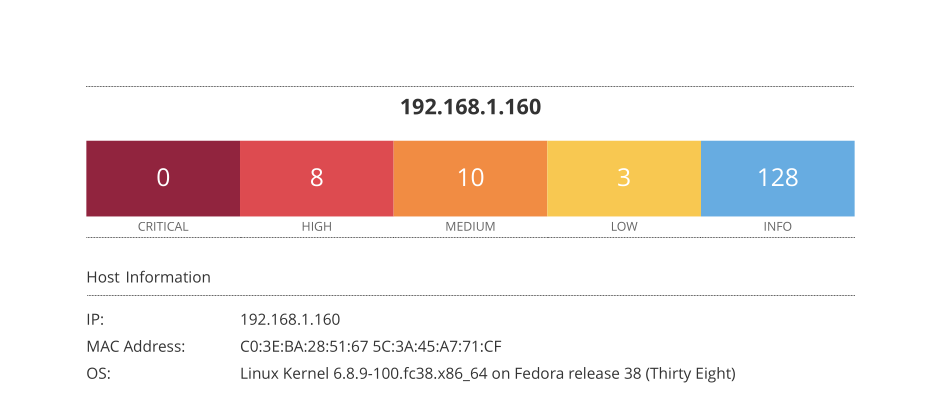
\includegraphics[scale=0.5]{imagenes/Capturas/11.png}
\end{figure}
\begin{figure}[H]
	\centering
	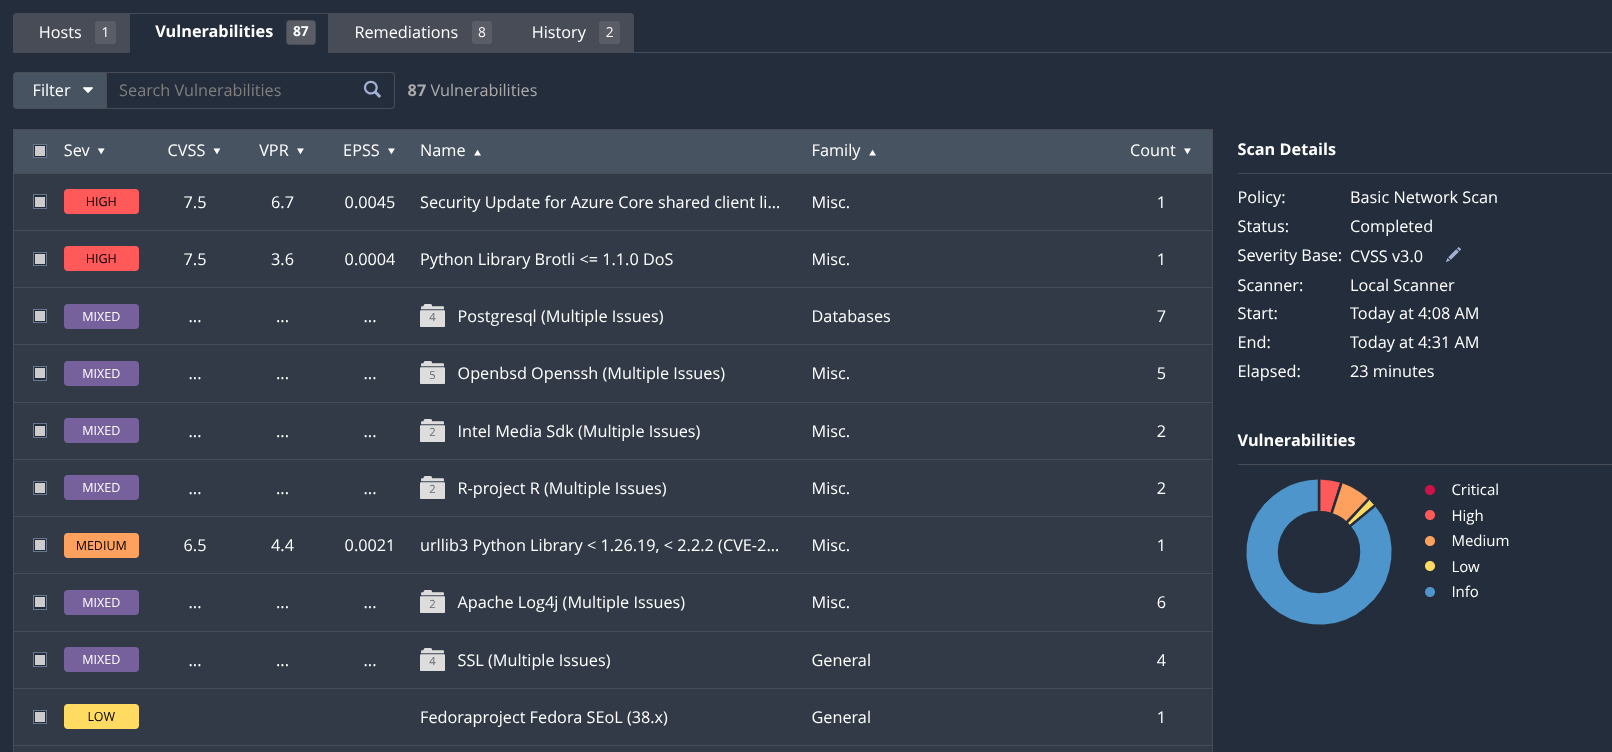
\includegraphics[scale=0.3]{imagenes/Capturas/12.png}
\end{figure}

Los resultados detallados de este escaneo se encuentran en el archivo \texttt{\textbf{Descubrimiento de Vulnerabilidades.pdf}}

\subsection{Soluciones a implementar}
A continuación se realizan diferentes métodos para solucionar estas vulnerabilidades encontradas. Las agruparemos por software o servicio. Se usa Gemini para analizar las vulnerabilidades y encontrar la solución adecuada.
\begin{enumerate}
	\item \textbf{Fedoraproject Fedora SEoL (201358)}
	\begin{figure}[H]
		\vspace{-10pt}
		\centering
		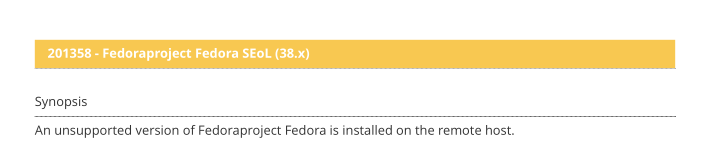
\includegraphics[scale=0.7]{imagenes/Capturas/2-13.png}
		\vspace{-30pt}
	\end{figure}
	Fedora 38 llegó a su fin de vida en 2024, lo que significa que actualmente no recibe parches de seguridad ni actualizaciones de aplicaciones. La solución que se implementará, será actualizar el SO de Fedora 38 a Fedora 42 (última versión estable y soportada). \\
	Para minimizar riesgos, la recomendación general es no saltar más de dos versiones a la vez, por lo se instala primero Fedora 40, para luego instalar Fedora 42. 
	
	\begin{enumerate}
		\item  Primero, actualizamos lo más posible la versión actual:
		\begin{verbatim}
			sudo dnf upgrade --refresh
		\end{verbatim}
	
		\item  Descargaremos los paquetes para la versión 40. Usaremos --allowerasing para que el gestor resuelva conflictos eliminando paquetes antiguos si es necesario:
		\begin{verbatim}
			sudo dnf system-upgrade download --releasever=40 --allowerasing
		\end{verbatim}
	
		\item  Ejecutamos el reinicio y actualización:
		\begin{verbatim}
			sudo dnf system-upgrade reboot
		\end{verbatim}
		
		\item  Verificamos la versión:
		\begin{verbatim}
			cat /etc/fedora-release
		\end{verbatim}
		\begin{figure}[H]
			\centering
			\vspace{-20pt}
			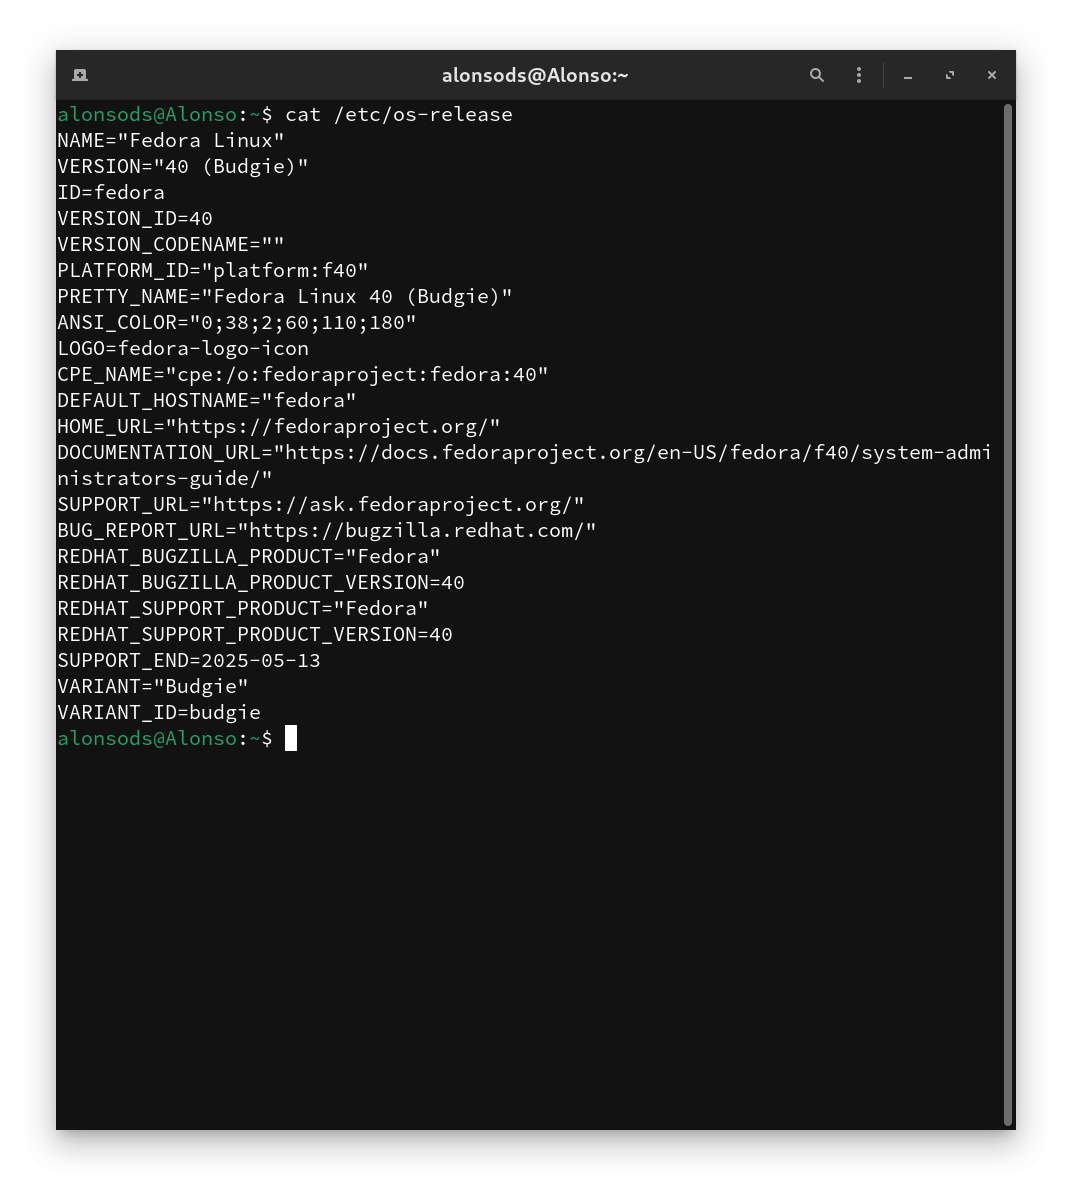
\includegraphics[scale=0.35]{imagenes/Capturas/s1-1.png}
			\vspace{-30pt}
		\end{figure}
		
		\item  Limpiamos archivos restantes de la descarga anterior y liberamos espacio:
		\begin{verbatim}
			sudo dnf system-upgrade clean
			sudo dnf clean all
		\end{verbatim}
		
		\item Ahora repetiremos todos los pasos anteriores en ese mismo orden, cambiando solo el número de versión:
		\begin{verbatim}
			sudo dnf system-upgrade download --releasever=42 --allowerasing
		\end{verbatim}
		\begin{figure}[H]
			\centering
			\vspace{-20pt}
			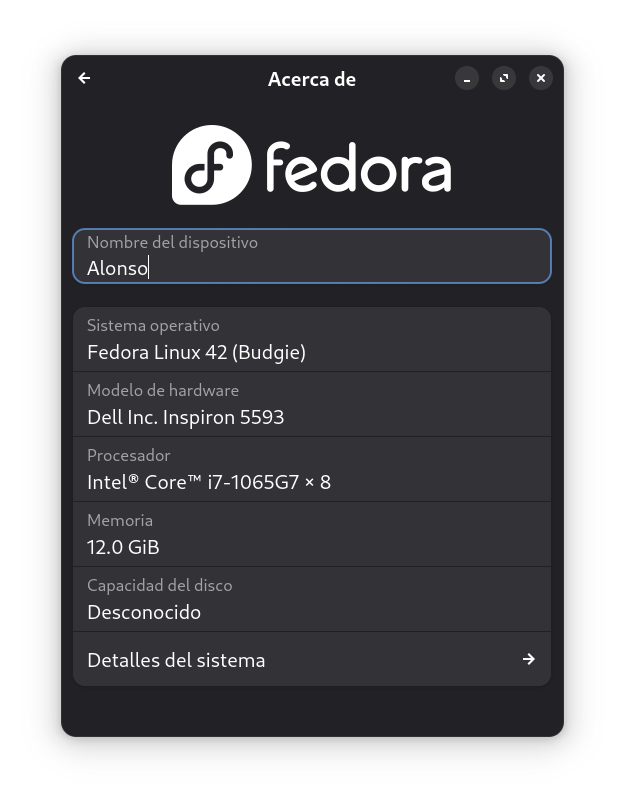
\includegraphics[scale=0.5]{imagenes/Capturas/s1-2.png}
			\vspace{-30pt}
		\end{figure}
	\end{enumerate}
	
	\item \textbf{OpenSSH (201194, 187201, 234554, 269984)}
	\begin{figure}[H]
		\vspace{-10pt}
		\centering
		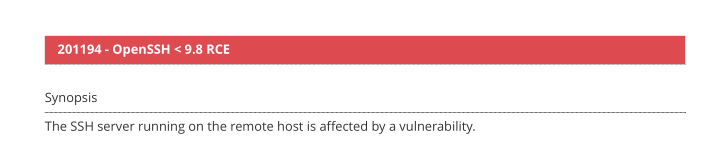
\includegraphics[scale=0.7]{imagenes/Capturas/2-2.png}
		\vspace{-30pt}
	\end{figure}
	\begin{figure}[H]
		\vspace{-10pt}
		\centering
		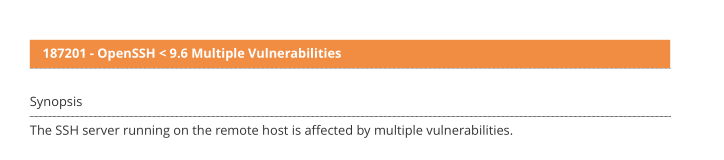
\includegraphics[scale=0.7]{imagenes/Capturas/2-9.png}
		\vspace{-30pt}
	\end{figure}
	\begin{figure}[H]
		\vspace{-10pt}
		\centering
		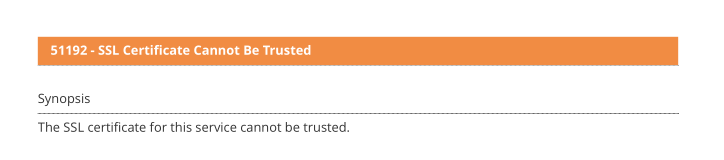
\includegraphics[scale=0.7]{imagenes/Capturas/2-11.png}
		\vspace{-30pt}
	\end{figure}
	\begin{figure}[H]
		\vspace{-10pt}
		\centering
		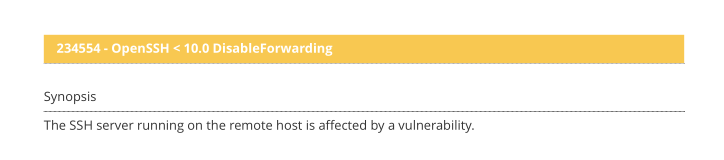
\includegraphics[scale=0.7]{imagenes/Capturas/2-14.png}
		\vspace{-30pt}
	\end{figure}
	\begin{figure}[H]
		\vspace{-10pt}
		\centering
		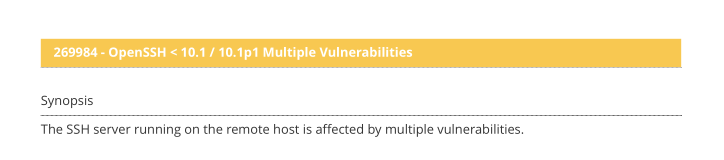
\includegraphics[scale=0.7]{imagenes/Capturas/2-15.png}
		\vspace{-30pt}
	\end{figure}
	Se tiene versiones vulnerables. Nessus recomienda llegar a la versión 10.1. La solución es actualizar los archivos del servidor SSH y reiniciar el servicio para que cargue la nueva versión en memoria.
	\begin{verbatim}
		sudo dnf upgrade openssh-server openssh-clients
		sudo systemctl restart sshd
	\end{verbatim}
	\begin{figure}[H]
		\centering
		\vspace{-20pt}
		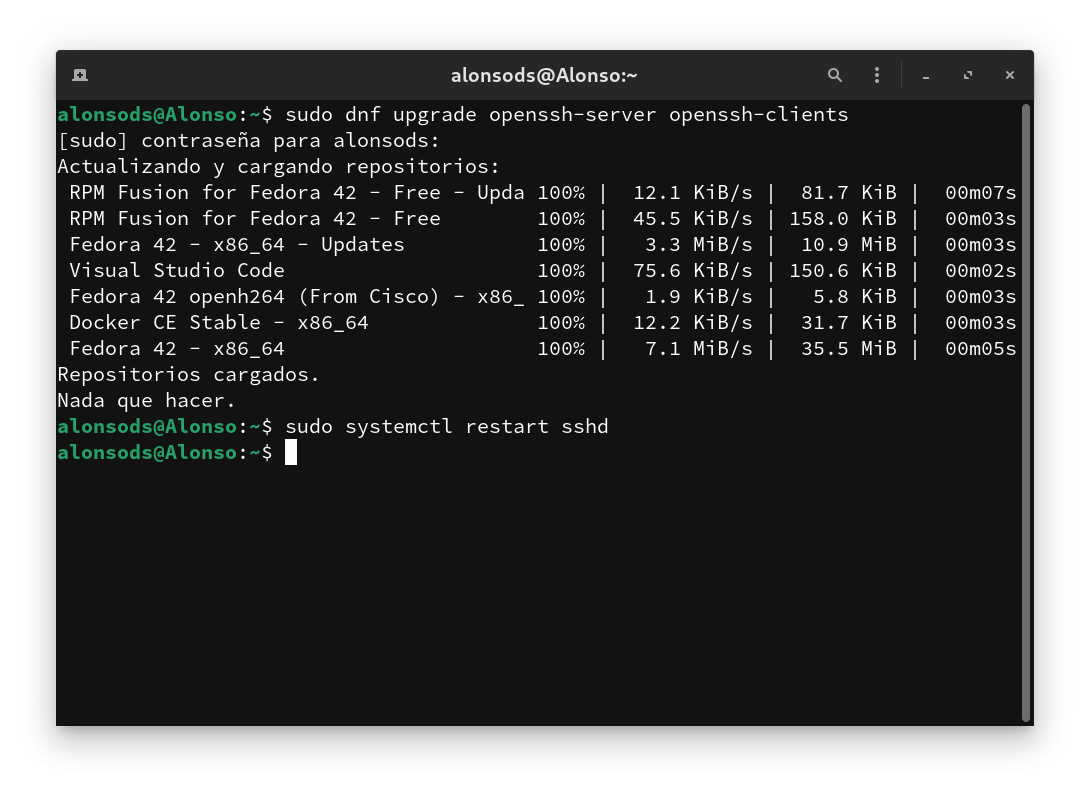
\includegraphics[scale=0.35]{imagenes/Capturas/s2-1.png}
		\vspace{-30pt}
	\end{figure}
	
	\item \textbf{PostgreSQL (299758, 299757, 275842)}
	\begin{figure}[H]
		\vspace{-10pt}
		\centering
		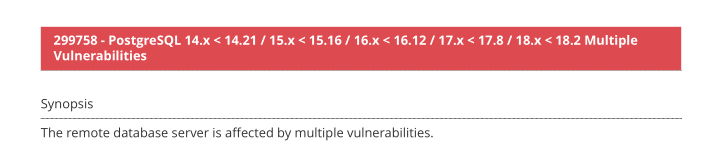
\includegraphics[scale=0.7]{imagenes/Capturas/2-3.png}
		\vspace{-30pt}
	\end{figure}
	\begin{figure}[H]
		\vspace{-10pt}
		\centering
		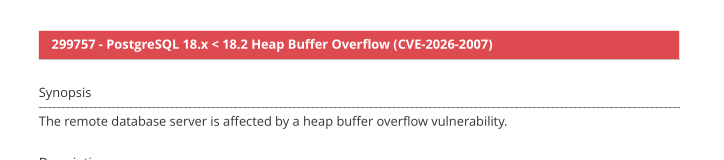
\includegraphics[scale=0.7]{imagenes/Capturas/2-4.png}
		\vspace{-30pt}
	\end{figure}
	\begin{figure}[H]
		\vspace{-10pt}
		\centering
		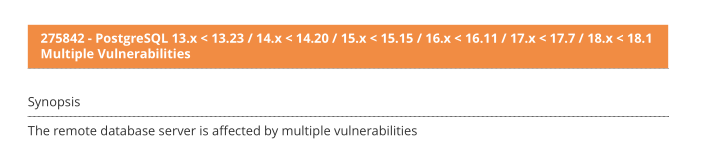
\includegraphics[scale=0.7]{imagenes/Capturas/2-10.png}
		\vspace{-30pt}
	\end{figure}
	Se encontraron múltiples vectores de desbordamiento de memoria (Heap Buffer Overflow) y vulnerabilidades de denegación de servicio asociadas a las extensiones y funciones del cliente \texttt{libpq}.
	La solución es actualizar la base de datos y sus librerias:
	\begin{verbatim}
		sudo dnf upgrade postgresql postgresql-server libpq
	\end{verbatim}
	Sin embargo al ejecutar el comando, el gesto \texttt{dnf} nos menciona que queremos actualizar \texttt{upgrade} al parque \texttt{postgresql-server} pero ese paquete ya no existe. ¿Entonces porqué se marcó como vulnerabilidad? Nessus es muy minucioso, por lo que pudo haber detectado las librerías cliente de PostgreSQL que se instalan como dependencias para otros programas. Nessus leyó la versión y lanzó alerta. \\
	Dado que el servidor no está instalado, simplemente lo omitimos de la actualización. Ejecuta el comando solo con los paquetes existentes:
	\begin{verbatim}
		sudo dnf upgrade postgresql libpq
	\end{verbatim}
	\begin{figure}[H]
		\centering
		\vspace{-20pt}
		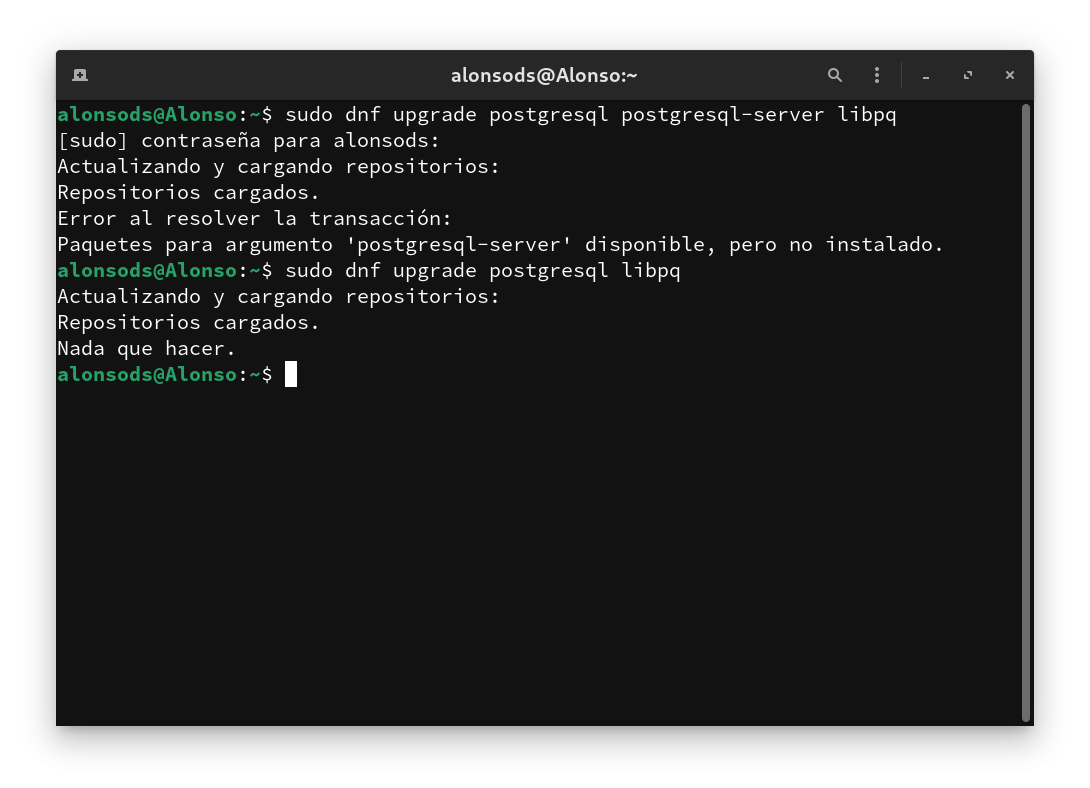
\includegraphics[scale=0.35]{imagenes/Capturas/s3-1.png}
		\vspace{-30pt}
	\end{figure}
	
	\item \textbf{Python: \texttt{brotli}, \texttt{urllib3}, azure-core (274433, 200807, 283875)}
	\begin{figure}[H]
		\vspace{-10pt}
		\centering
		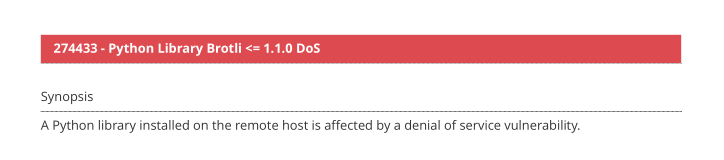
\includegraphics[scale=0.7]{imagenes/Capturas/2-5.png}
		\vspace{-30pt}
	\end{figure}
	\begin{figure}[H]
		\vspace{-10pt}
		\centering
		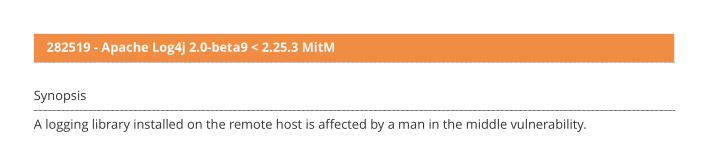
\includegraphics[scale=0.7]{imagenes/Capturas/2-8.png}
		\vspace{-30pt}
	\end{figure}
	\begin{figure}[H]
		\vspace{-10pt}
		\centering
		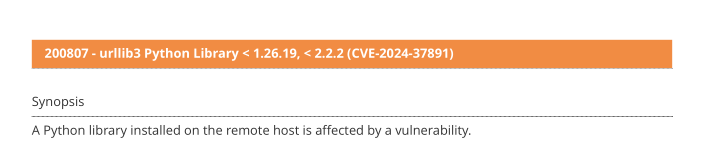
\includegraphics[scale=0.7]{imagenes/Capturas/2-12.png}
		\vspace{-30pt}
	\end{figure}
	Riesgos de denegación de servicio (DoS) por compresión en brotli, cabeceras proxy mal manejadas en urllib3 y escalada de privilegios en el SDK de Azure. \\
	Dado que estos suelen gestionarse a través de Python, lo ideal es usar \texttt{pip} para forzar la actualización a las versiones seguras que pide Nessus (ej. brotli 1.2.0+, urllib3 2.2.2+). Realizamos el siguiente comando:
	\begin{verbatim}
		pip install --upgrade brotli urllib3 azure-core
	\end{verbatim}
	\begin{figure}[H]
		\centering
		\vspace{-20pt}
		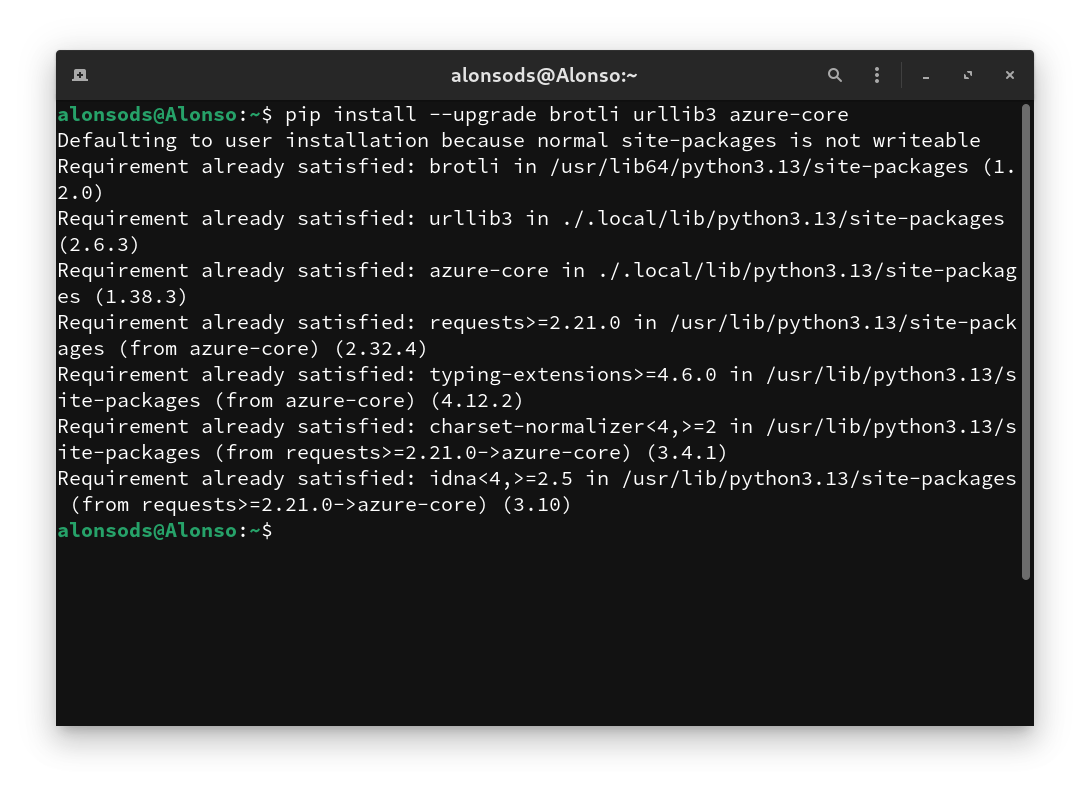
\includegraphics[scale=0.35]{imagenes/Capturas/s4-1.png}
		\vspace{-30pt}
	\end{figure}
	
	\item \textbf{Intel Media SDK (197900)}
	\begin{figure}[H]
		\vspace{-10pt}
		\centering
		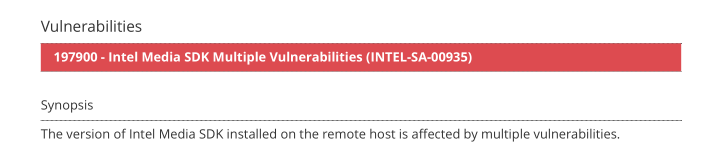
\includegraphics[scale=0.7]{imagenes/Capturas/2-1.png}
		\vspace{-30pt}
	\end{figure}
	Múltiples fallos de lectura/escritura fuera de límites y validación de entrada. En particular, el paquete intel-mediasdk (que contiene librerías como libmfx) es un kit de desarrollo de software creado por Intel. Su propósito era permitir que las aplicaciones aprovecharan la aceleración por hardware (Intel Quick Sync Video) para codificar, decodificar y procesar video. Intel descontinuó oficialmente este SDK. De hecho, la propia recomendación de seguridad de Intel para estas vulnerabilidades es desinstalarlo, ya que lo reemplazaron por una tecnología más moderna llamada Intel oneVPL. Por lo cual procedemos a desinstarlo:
	\begin{verbatim}
		sudo dnf remove intel-mediasdk
	\end{verbatim}
	\begin{figure}[H]
		\centering
		\vspace{-15pt}
		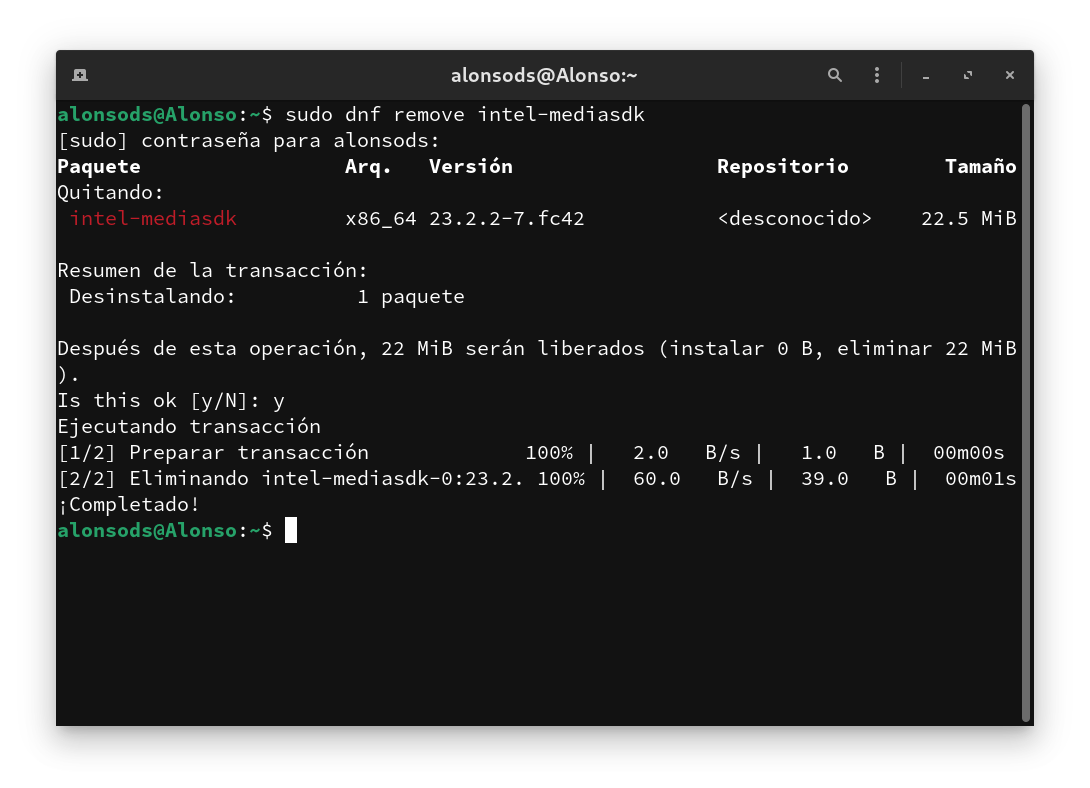
\includegraphics[scale=0.35]{imagenes/Capturas/s5-1.png}
		\vspace{-30pt}
	\end{figure}
	\newpage
	\item \textbf{Certificado SSL no confiable en puerto 8834 (51192)}
	\begin{figure}[H]
		\vspace{-10pt}
		\centering
		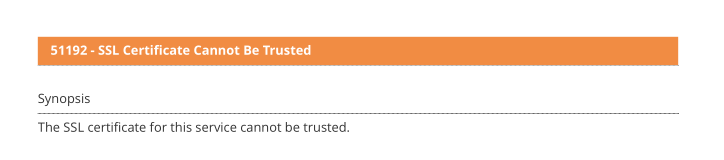
\includegraphics[scale=0.7]{imagenes/Capturas/2-11.png}
		\vspace{-30pt}
	\end{figure}
	El puerto 8834 es el que utiliza el propio Nessus Essentials. Al instalarlo, generó un certificado "autofirmado" para poder ofrecer acceso por HTTPS en localhost. Como no fue emitido por una entidad certificadora global, Nessus se detecta a sí mismo como inseguro. Por lo tanto, no hay soluciones que implementar. 
\end{enumerate}

\subsection{Segundo escaneo}
Cuando se hizo la actualización del sistema operativo de Fedora 38 a Fedora 42, ocurrió un cambio de IP local. La interfaz de red se reinició, y el router le asignó a la computadora una nueva dirección IP: \texttt{192.168.1.112}.
\begin{figure}[H]
	\centering
	\vspace{-15pt}
	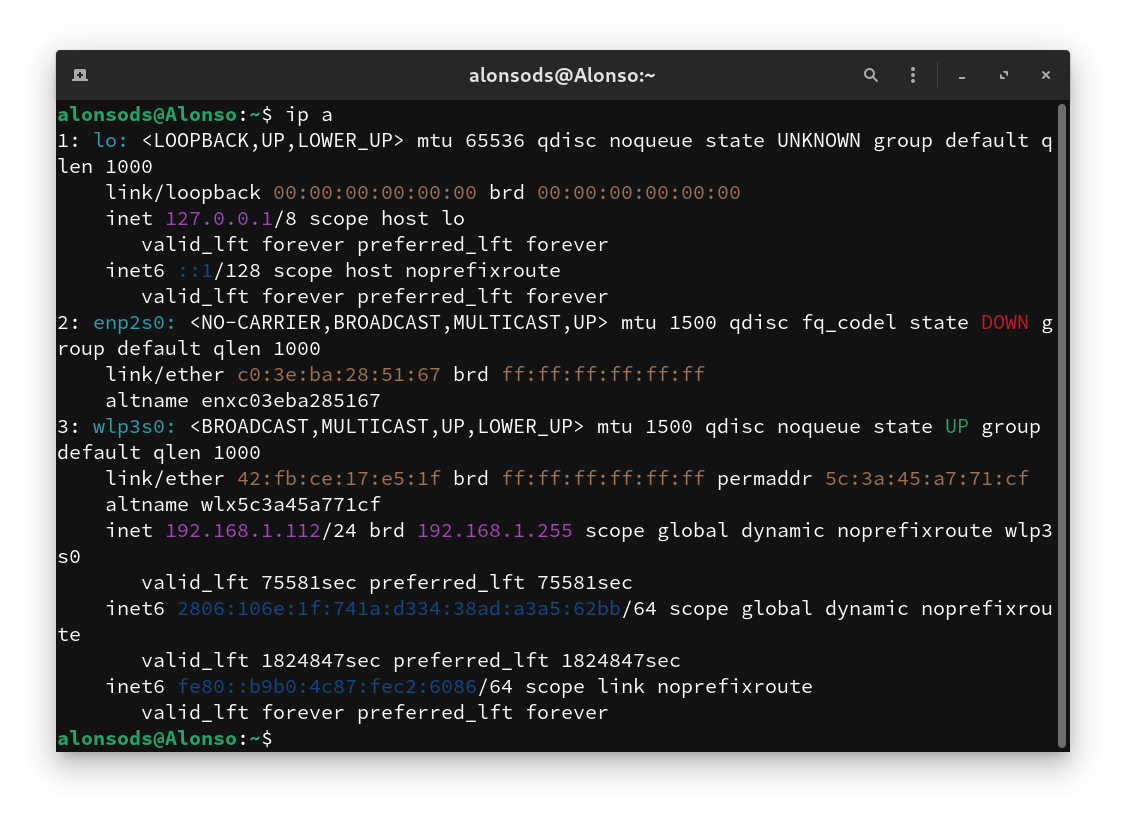
\includegraphics[scale=0.4]{imagenes/Capturas/3-1.png}
	\vspace{-30pt}
\end{figure}
Por lo tanto, actualizamos el objetivo a Nessus y ejecutamos un nuevo escaneo.
\begin{figure}[H]
	\centering
	\vspace{-15pt}
	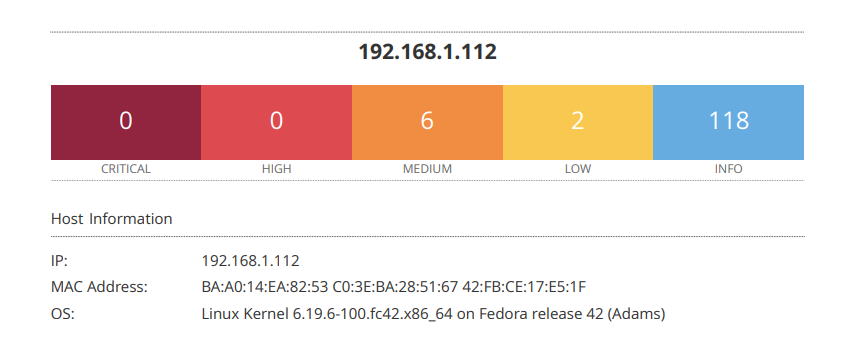
\includegraphics[scale=0.55]{imagenes/Capturas/e1.png}
	\vspace{-30pt}
\end{figure}

Los resultados detallados de este escaneo se encuentran en el archivo \texttt{\textbf{Descubrimiento de Vulnerabilidades (Post-medidas).pdf}}

\section{Vulnerabilidad: CVE-2014-0160}
Esta es una de las vulnerabilidades más conocidas de la historia de la ciberseguridad. Su nombre es ``Heartbleed'' (hemorragia de corazón). Afectó a la biblioteca criptográfica OpenSSL, específicamente a la implementación de la extensión "Heartbeat" (Latido de corazón) de TLS/DTLS. Sus parámetros CVSS son:
\begin{itemize}
	\item Puntuación CVSS v2: 5.0 (Media). Aunque la industria la trata como crítica por su facilidad de explotación.
	\item Vector de Acceso (AV): Red (Network). El atacante puede explotarla remotamente desde internet.
	\item Complejidad de Acceso (AC): Baja. Es trivial de explotar; no requiere condiciones especiales en el sistema.
	\item Autenticación (Au): Ninguna. El atacante no necesita credenciales para explotarla.
	\item Impacto de Confidencialidad (C): Parcial.
	\item Impacto de Integridad y Disponibilidad: Ninguno. El ataque no modifica ni tira el servicio, solo lee datos sigilosamente.
\end{itemize}
La falla consistía en un error de comprobación de límites (Buffer Over-read). Un atacante enviaba un mensaje al servidor engañándolo sobre el tamaño del mensaje. El servidor, al responder, devolvía el mensaje original más un fragmento de su propia memoria RAM (hasta 64 kilobytes por intento). \\
Su manera de ataque es filtrar claves privadas maestras X.509 del servidor, nombres de usuario, contraseñas en texto plano, cookies de sesión de los usuarios conectados y correos electrónicos que estuvieran pasando por la RAM en ese momento. \\
Comprometió la seguridad de casi el 20\% de los servidores web seguros de todo internet en 2014, obligando a revocar masivamente certificados SSL y a los usuarios a cambiar sus contraseñas en plataformas globales.